In 2010, the dijet \pt{} balance method was not used to recalibrate the jets, but was used to assess the uncertainty on the JES calibration factors.
However, the relative jet response \cite{ref:EtaInter2010} shows a difference in the forward region for MC and data.
The difference between the data and MC jet responses could either originate from physics or the detector effects described in Section \ref{sec:Det:Jets}. 
Until the source of the differences is determined, these relative response factors should not be used to calibrate the jets for physics analysis.
However, they are used to test the closure of the calibration and to see the difference between data and MC can be resolved.

Using the ratio of the relative response factors from the MC and the data, the residual correction, 

\begin{equation}
\mathcal{C_{\rm{in-situ}}} = \frac{\rm{c_{MC}}}{\rm{c_{Data}}}
\label{JetPerf:ResidualCorrection}
\end{equation}
is calculated, where ${1}/{\rm{c_{MC}}}$ and ${1}/{\rm{c_{Data}}}$ are the relative response factors for MC and data, respectively. 


Figure \ref{JetPerf:EtaData} shows the jet $\eta$ distribution for (a) \pt{} $>30$ GeV from the Min Bias trigger and (b) \pt{}$>50$ GeV from the calorimeter trigger stream. 
The in-situ calibrated data has a much better agreement with the MC than the uncorrected data in both plots. 
There are still differences in the forward region, but overall the differences are smaller than $10\%$.

Figure \ref{JetPerf:E_PtData} shows (a) the jet energy  and  (b) the \pt{} distributions  for jets in the region \etaRange{3.2}{4.5}  for \pt{}$>20$ GeV. 
The energy distribution shows improvements in agreement between the MC after the data has been calibrated.
The \pt{} distribution shows smaller differences for the in-situ calibrated data.

These results show that calibration brings the data into  closer agreement with the MC, giving confidence to the method and the results.
This confidence resulted in the decision to use the dijet \pt{} balance method to calibrate the jets in the 2011 sample. 
These plots were published in an ATLAS conference note \cite{ref:EtaInter2010}.

\begin{figure}
\centering
        \begin{subfigure}[b]{0.5\textwidth}
                \centering
                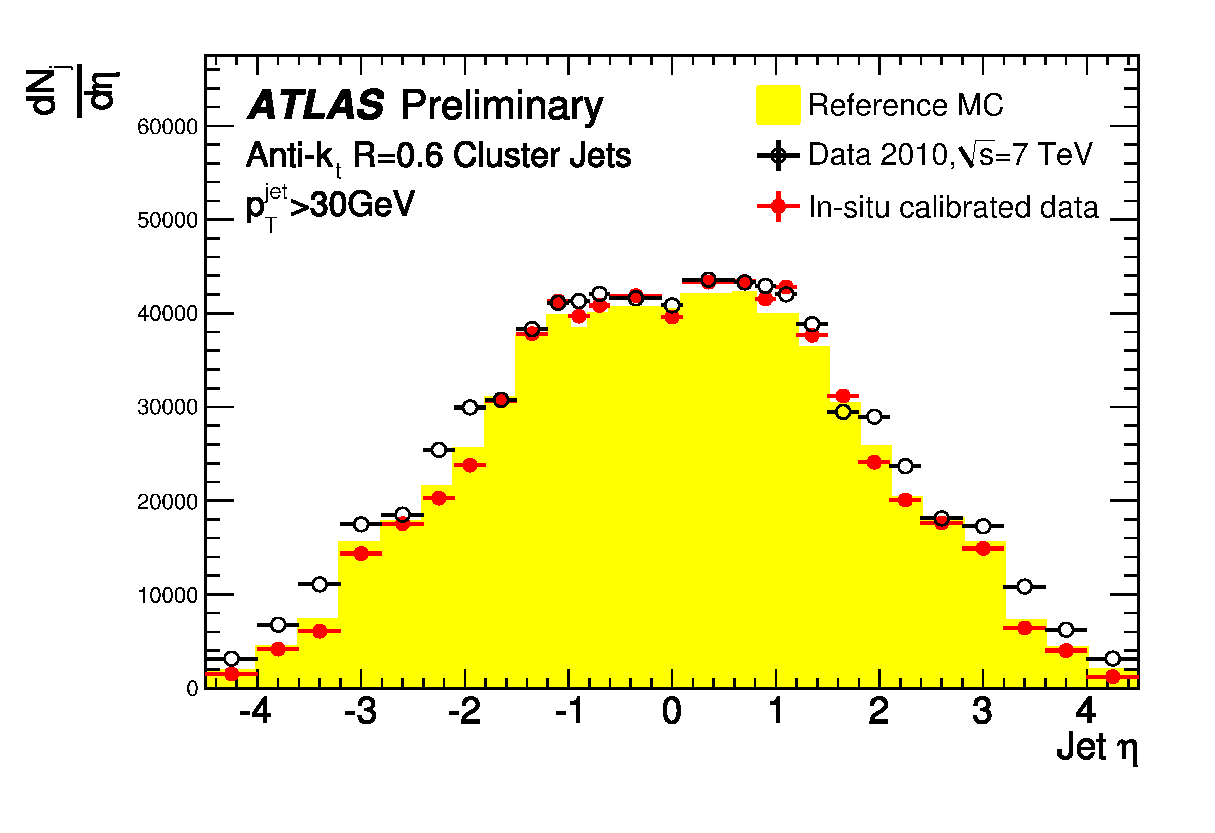
\includegraphics[width=\textwidth]{figures/JetPerformance/EtaDist30GeV.eps}
        \end{subfigure}%
        \begin{subfigure}[b]{0.5\textwidth}
                \centering
                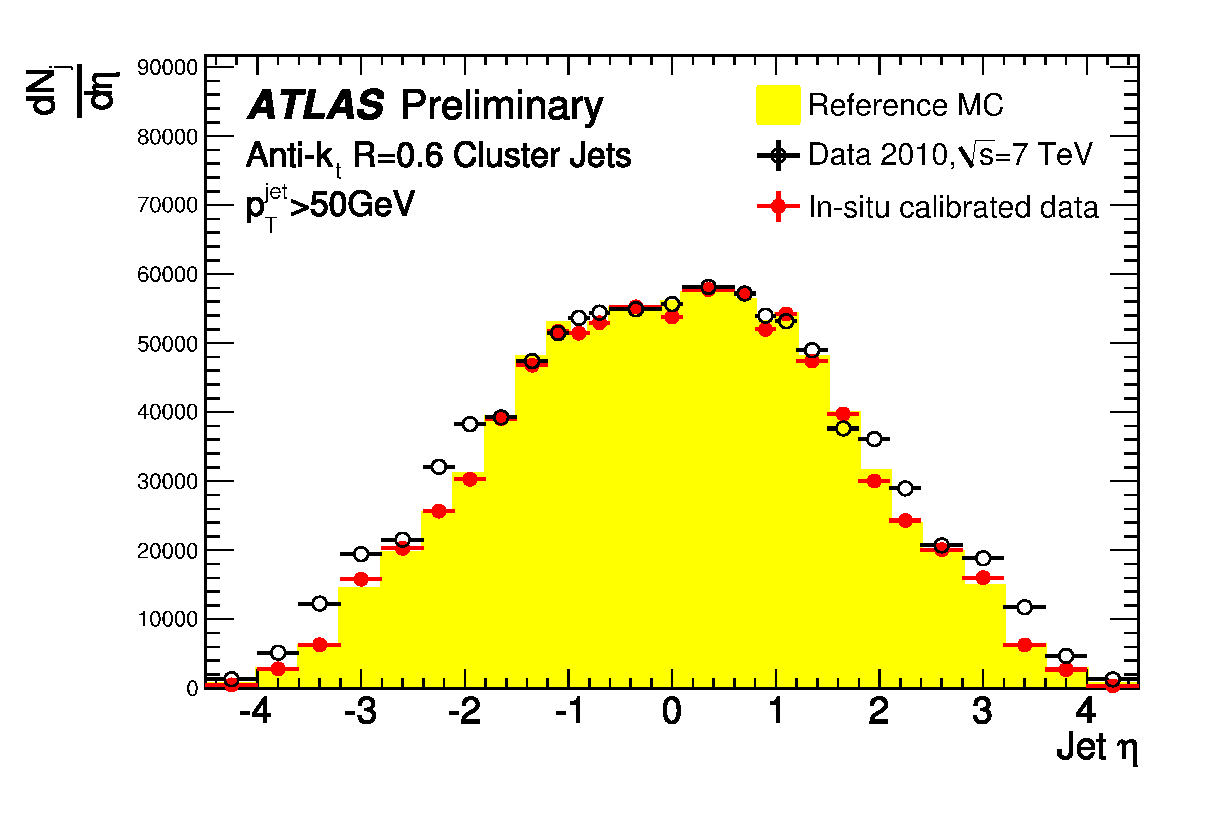
\includegraphics[width=\textwidth]{figures/JetPerformance/EtaDist50GeV.eps}
        \end{subfigure}%
\caption[Effect of additional calibration on the jet $\eta$ distribution]{
$\eta$ distribution for jets with (a) \pt{} $>30$ GeV from the Min Bias trigger and (b) \pt{} $>50$ GeV from the calorimeter trigger stream. 
Uncorrected data (open black circles) and corrected data (red circles) are shown along with the reference MC. 
\label{JetPerf:EtaData}}
%\end{figure}
\medskip
%\begin{figure}
        \begin{subfigure}[b]{0.5\textwidth}
                \centering
                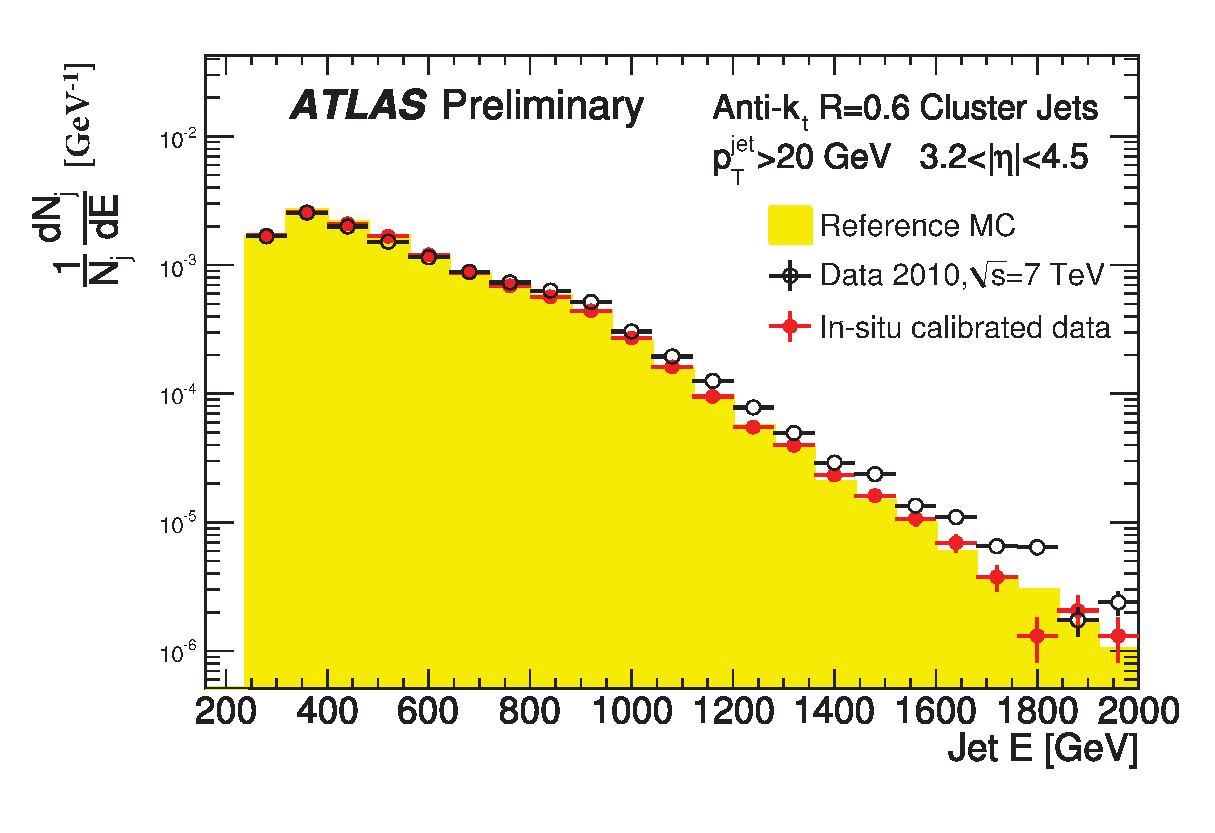
\includegraphics[width=\textwidth]{figures/JetPerformance/EDist-Edit.eps}
        \end{subfigure}%
        \begin{subfigure}[b]{0.5\textwidth}
                \centering
                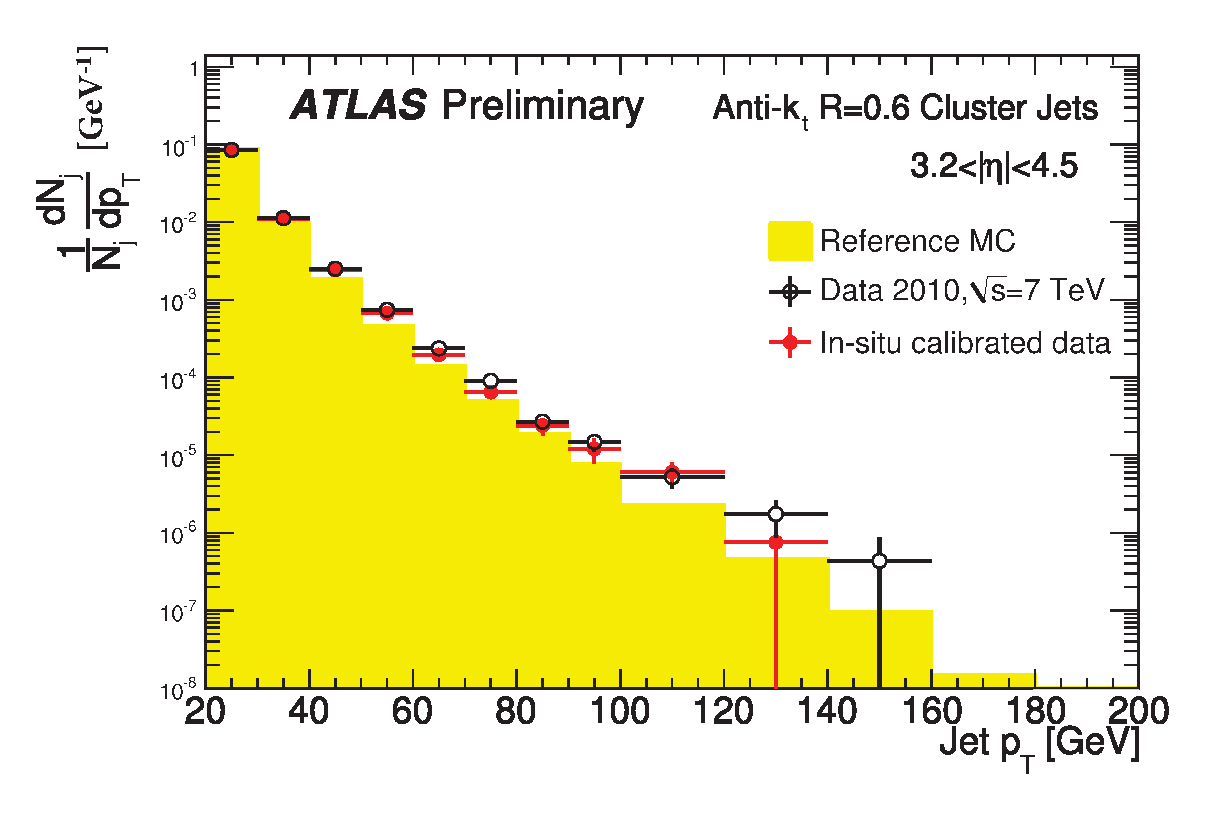
\includegraphics[width=\textwidth]{figures/JetPerformance/PtDist-Edit.eps}
        \end{subfigure}%
\caption[Effect of additional calibration on the jet energy and \pt{} distributions for jets in the FCal]{
(a) Jet energy and (b) jet \pt{} for the region \etaRange{3.2}{4.5}.
Uncorrected data (open black circles) and corrected data (red circles) are shown along with the reference MC. 
\label{JetPerf:E_PtData}}
\end{figure}
